\documentclass[a4paper, 12pt, final, garamond]{book}
\usepackage{cours-preambule}

\raggedbottom

\makeatletter
\renewcommand{\@chapapp}{M\'ecanique -- chapitre}
\makeatother

\toggletrue{student}
% % \HideSolutionstrue
% \toggletrue{corrige}
\renewcommand{\mycol}{black}
% \renewcommand{\mycol}{gray}

\begin{document}
\setcounter{chapter}{2}

\chapter{\cswitch{Correction du TD}{TD application~: mouvements courbes}}

\resetQ
\section{Projection de vecteurs}
\QR{%
	Exprimer $\vfo$ dans la base $(\ux,\uz)$ en fonction de $v_0$ et
	$\a$.
	\begin{center}
		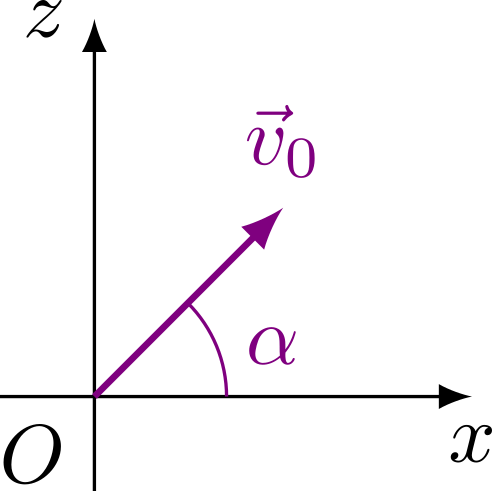
\includegraphics[scale=1]{vec_a}
	\end{center}
}{%
	Si $\a$ vaut 0, $\vfo$ est selon $\ux$. On sait donc que la
	projection de $\vfo$ sur $\ux$ donne $v_0\cos\a\ux$. On le remarque
	également avec le triangle rectangle OMH, avec M le bout de $\vfo$ et H
	son projeté orthogonal sur $\ux$~: la longueur OH est en effet
	$v_0\cos\a$. \bigbreak
	Si $\a$ vaut $\pi/2$, $\vfo$ est selon $\uz$. On sait donc que la
	projection de $\vfo$ sur $\uz$ donne $v_0\sin\a\uz$. On le remarque
	également en prenant le triangle rectangle OMJ, avec cette fois J le
	projeté orthogonal de M sur $\uz$~: la longueur OJ est en effet
	$v_0\sin\a$. Finalement,
	\[\boxed{\vfo = v_0\cos\a\ux + v_0\sin\a\uz}\]
}
\QR{%
	Exprimer $\Nf$ et $\Tf$ dans la base $(\ux,\uz)$ en fonction de $N$,
	$T$ et $\a$.
	\begin{center}
		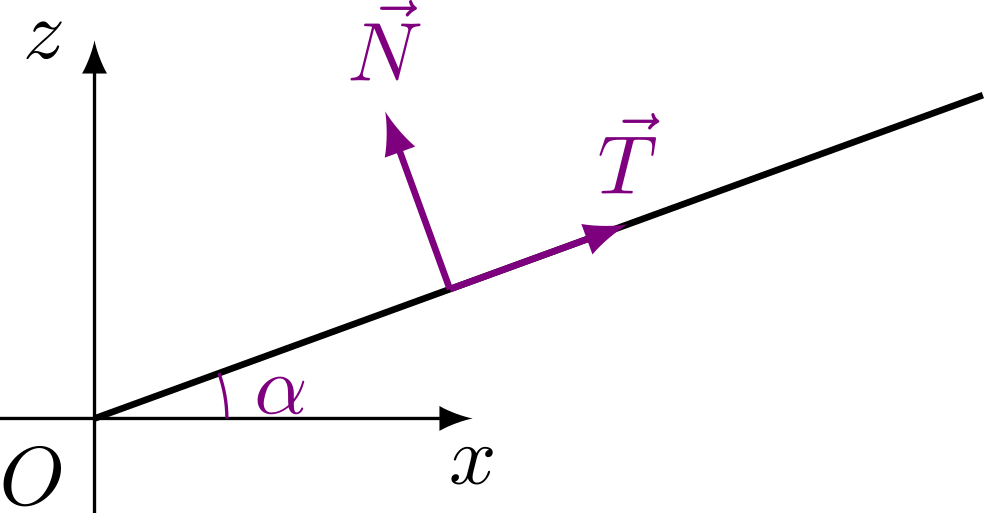
\includegraphics[scale=1]{vec_b}
	\end{center}
}{%
	Avec la même réflexion, on trouve
	\[\boxed{\Tf = T\cos\a\ux + T\sin\a\uz}\]
	La méthode est la même pour $\Nf$, mais le résultat est différent. En
	effet, si $\a = 0$, $\Nf$ est selon $\uz$~: la projection de $\Nf$ sur
	$\uz$ donne $N\cos\a\uz$. Si $\a = \pi/2$, $\Nf$ est selon $-\ux$~: la
	projection de $\Nf$ sur $\ux$ donne $-N\sin\a\ux$. Ainsi,
	\[\boxed{\Nf = -N\sin\a\ux + N\cos\a\uz}\]
}
\QR{%
	Exprimer $\Pf$ et $\Tf$ dans la base $(\er,\et)$ en fonction de $m$,
	$g$, $T$ et $\tt$.
	\begin{center}
		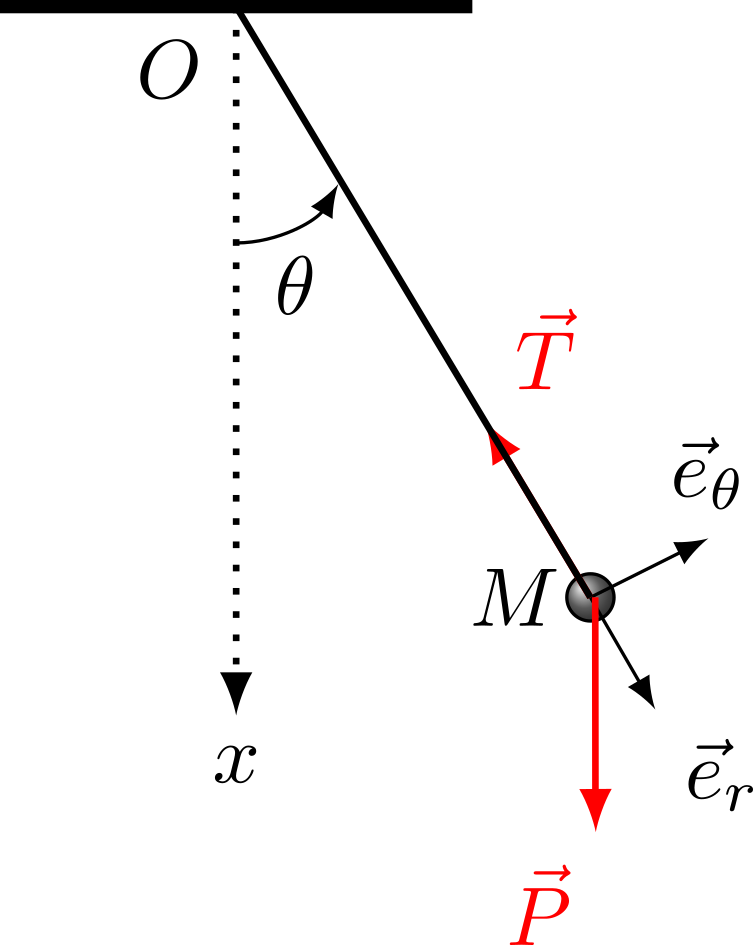
\includegraphics[scale=1]{vec_c}
	\end{center}
}{%
	Toujours même réflexion~: si $\tt = 0$, $\Pf$ est selon $\er$, et si
	$\tt = \pi/2$, $\Pf$ est selon $-\et$. $\Tf$ est, par définition, selon
	$-\er$. Ainsi,

	\[
		\boxed{\Pf = mg\cos\tt\er -mg\sin\tt\et}
		\qet
		\boxed{\Tf = -T\er}
	\]
}
\QR{%
	\textbf{Équilibre plan incliné}
	À l'équilibre des forces, on a
	\[\Nf + \Tf + \Pf = \of\]
	Projeter le poids dans la base inclinée et exprimer les normes de $\Tf$
	et $\Nf$ en fonction de $m$, $g$ et $\a$.
	\begin{center}
		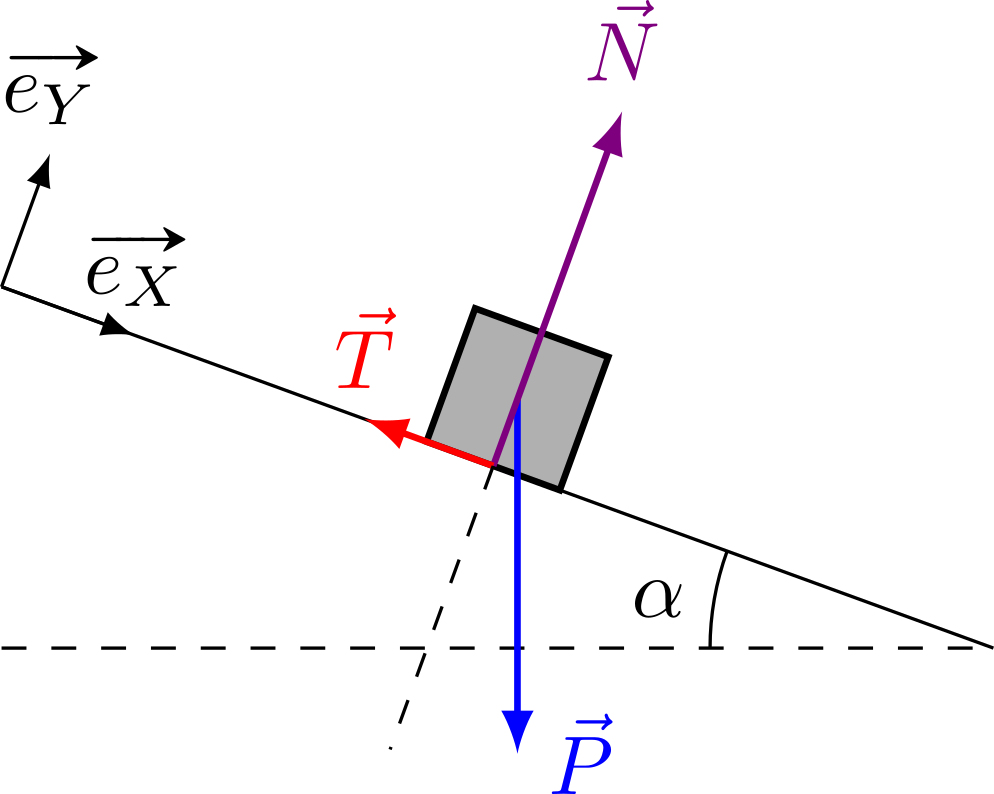
\includegraphics[scale=1]{vec_d}
	\end{center}
}{%
	Ici aussi~:
	\begin{itemize}
		\item $\a = 0 \Ra \Pf\cdot\vv{e_Y} = -1
			      \quad
			      \text{($\Pf$ selon $-\vv{e_Y}$)}$
		\item $\a = \pi/2 \Ra
			      \Pf\cdot\vv{e_X} = 1
			      \quad
			      \text{($\Pf$ selon $\vv{e_X}$)}$
	\end{itemize}
	Ainsi
	\[
		\boxed{\Pf = mg(\sin\a\vv{e_X} -\cos\a\vv{e_Y})}
		\qet
		\boxed{\Nf = N\vv{e_Y}}
		\qet
		\boxed{\Tf = -T\vv{e_X}}
	\]
	D'où
	\[
		\Nf + \Tf + \Pf = \of
		\Lra
		\mqty(mg\sin\a -T\\-mg\cos\a + N) = \mqty(0\\0)
		\Lra
		\boxed{
			\left\{
			\begin{aligned}
				T & = mg\sin\a \\
				N & = mg\cos\a
			\end{aligned}
			\right.}
	\]
}
\QR{%
	\textbf{Équilibre hamac}
	À l'équilibre des forces, on a
	\[\Ff_g + \Ff_d + \Pf = \of\]
	Projeter les vecteurs $\Ff_g$ et $\Ff_d$ dans la base $(\ux,\uy)$ avec
	$\ux$ parallèle au sol vers la droite et $\uy$ vertical ascendant. En
	déduire la norme littérale de ces deux vecteurs. On prend $m =
		\SI{60}{kg}$, $\a = \ang{45}$ et $\beta = \ang{60}$.
	\begin{center}
		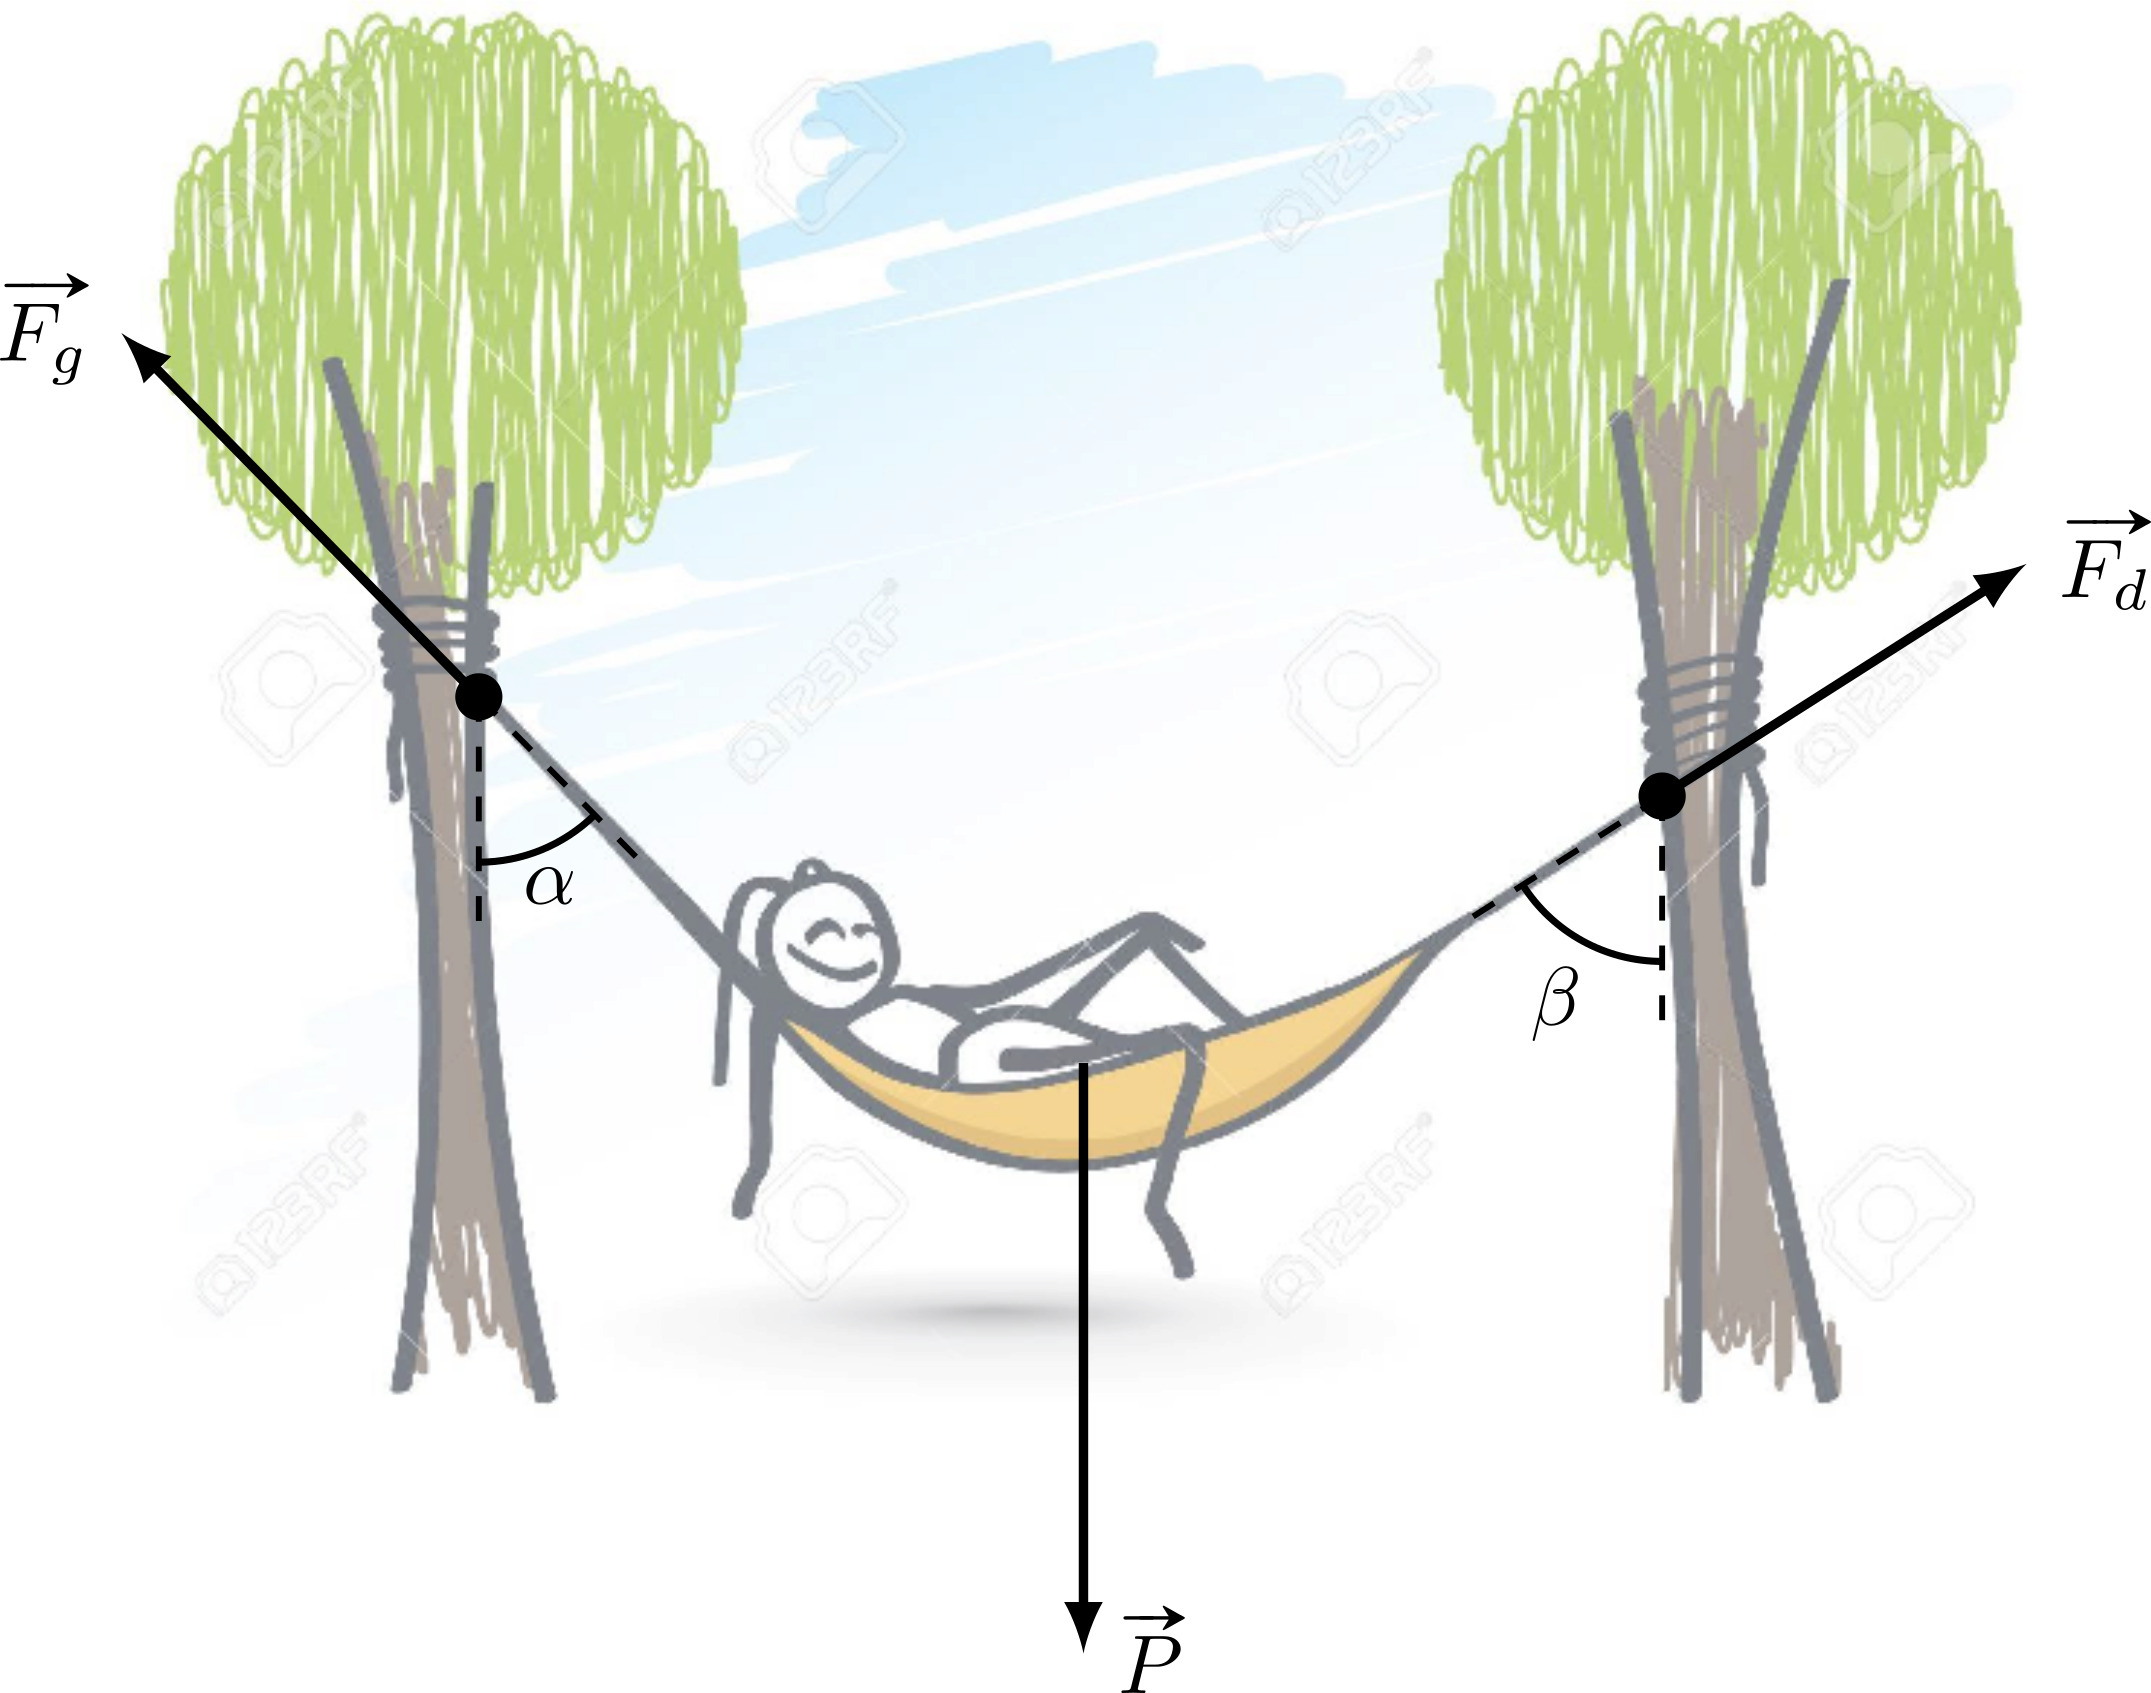
\includegraphics[scale=.7]{vec_e}
	\end{center}
}{%
	On projette~:
	\[
		\Ff_g = F_g(\cos\a\uy -\sin\a\ux)
		\qet
		\Ff_d = F_d(\cos\bb\uy+\sin\bb\ux)
	\]
	et avec l'égalité de vecteurs on obtient
	\begin{align*}
		\left\{
		\begin{aligned}
			0 & = F_d\sin\bb -F_g\sin\a      \\
			0 & = -mg+F_g\cos\a + F_d\cos\bb
		\end{aligned}
		\right.
		 & \Lra
		\left\{
		\begin{aligned}
			F_d & = F_g\frac{\sin\a}{\sin\bb}                    \\
			mg  & = F_g\cos\a + F_g\frac{\sin\a}{\sin\bb}\cos\bb
		\end{aligned}
		\right.
		\\\Lra
		\left\{
		\begin{aligned}
			F_d       & = F_g\frac{\sin\a}{\sin\bb}          \\
			mg\sin\bb & = F_g(\cos\a\sin\bb + \sin\a\cos\bb)
		\end{aligned}
		\right.
		 & \Lra
		\boxed{
			\left\{
			\begin{aligned}
				F_d & = \frac{mg\sin\a}{\cos\a\sin\bb + \sin\a\cos\bb}  \\
				F_g & = \frac{mg\sin\bb}{\cos\a\sin\bb + \sin\a\cos\bb}
			\end{aligned}
			\right.
		}
	\end{align*}
	Les applications numériques, \textbf{non demandées}, donnent
	\[
		\boxed{
			\left\{
			\begin{array}{rcl}
				F_d & = & \SI{4.4e2}{N} \\
				F_g & = & \SI{5.4e2}{N}
			\end{array}
			\right.
		}
	\]
}

\resetQ
\section{Masse du Soleil}
\enonce{%
	La Terre subit de la part du Soleil la force d'attraction gravitationnelle~:
	\[
		\Ff_g = -\Gc \frac{M_TM_S}{R^2}\ur
		\qMath{où}
		\Gc = \SI{6.67e-11}{SI}
	\]
	avec $\ur$ le vecteur unitaire allant du Soleil vers la Terre. La Terre tourne
	autour du Soleil en décrivant un cercle de rayon $R = \SI{149.6e6}{km}$.
}
\QR{%
	Déterminer la masse du Soleil.
}{%
	On étudie le système \{Terre\} dans le référentiel héliocentrique. La Terre
	étant sur une orbite circulaire, on utilise un repère polaire $({\rm
				S},\ur,\ut)$ en appelant S le centre de gravité du
	Soleil et T le centre de gravité de la Terre. On a~:
	\begin{gather*}
		\vv{\rm ST} = R\ur\\
		\vf = R\tp\ut\\
		\af = \underbrace{\cancel{R\tpp\ut}}_{\tpp=0} -R\tp^2\ur
	\end{gather*}
	étant donné que la distance Terre-Soleil est fixe, et que la vitesse angulaire
	de la Terre autour du Soleil est constante. On a d'ailleurs, en appelant $\w =
		\tp$ cette vitesse angulaire,
	\[\w = \frac{2\pi}{T_0}\]
	avec $T_0$ la période de révolution de la Terre autour du Soleil, telle que $T_0
		= \num{365.26}\times\num{24}\times{3600}\si{s} = \SI{3.16e7}{s}$. Ainsi, la
	seule force s'exerçant sur la Terre étant l'attraction gravitationnelle du
	Soleil, on a avec le PFD~:
	\begin{gather*}
		M_{T}\af = \Ff_g
		\Lra
		-\cancel{M_T}R\w^2 = -\Gc \frac{\cancel{M_T}M_S}{R^2}\\
		\Lra
		\boxed{M_S = \frac{R^3\w^2}{\Gc} = \frac{4\pi^2R^3}{\Gc T_0{}^2}}
		\qavec
		\left\{
		\begin{array}{rcl}
			R   & = & \SI{1.496e11}{m}  \\
			\Gc & = & \SI{6.67e-11}{SI} \\
			T_0 & = & \SI{3.16e7}{s}
		\end{array}
		\right.
		\Ra
		\boxed{M_S = \SI{1.99e30}{kg}}
	\end{gather*}
}

\resetQ
\section{Oscillations d'un anneau sur un cerceau}
\noindent
\begin{minipage}[c]{.74\linewidth}
	\enonce{%
		Un cerceau de centre O et de rayon $R$ est maintenu dans un plan vertical,
		et un anneau de masse $m$ assimilé à un point matériel M peut glisser sans
		frottements le long de ce cerceau.
	}
	\QR{%
		Qu'est-ce que l'hypothèse «~sans frottements~» implique pour la
		réaction du cerceau sur l'anneau~?
	}{%
		L'hypothèse «~sans frottements~» signifie que la réaction du cerceau
		est uniquement normale~: il n'y a pas de composante tangentielle.
	}
\end{minipage}
\begin{minipage}[c]{.25\linewidth}
	~
	\begin{center}
		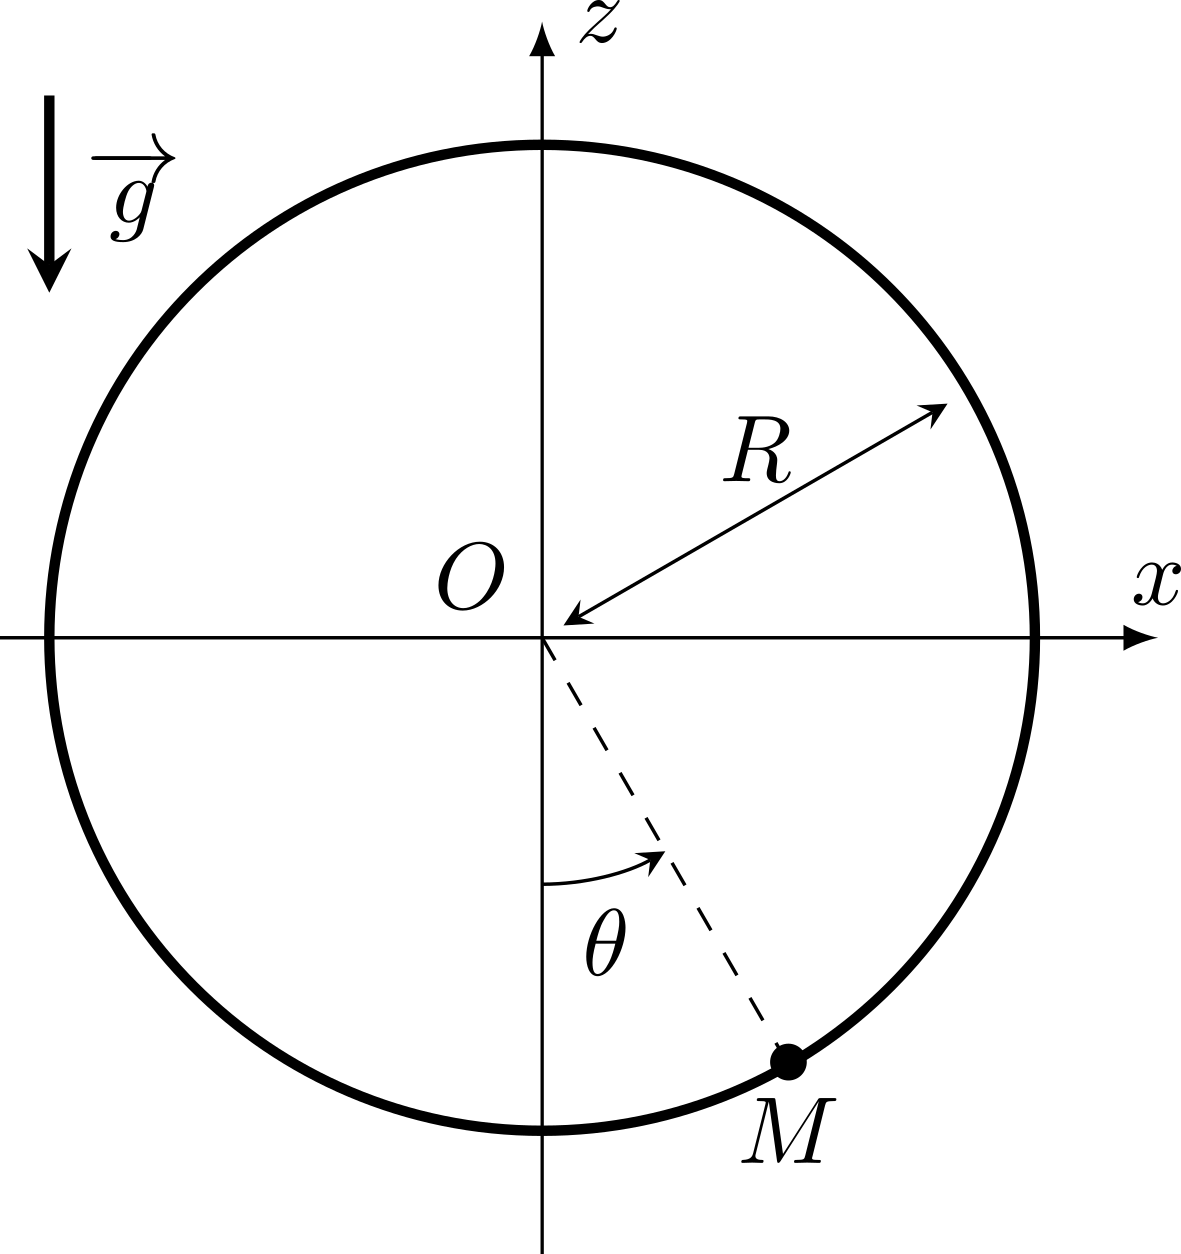
\includegraphics[width=\linewidth]{anneau_cerceau-plain}
	\end{center}
\end{minipage}

\QR<[start=2]>{%
	Écrire le PFD appliqué à l'anneau et le projeter dans une base
	adaptée.
}{%
	\begin{itemize}
		\bitem{Système~:} \{anneau\}
		\bitem{Référentiel~:} $\Rc\ind{sol}$ supposé galiléen
		\bitem{Repère~:} $(\Or,\ur,\ut)$ avec $\ut$ dans le sens de $\tt$
		\bitem{Repérage~:}
		\begin{align*}
			\OM(t) & = R\ur                 \\
			\vf(t) & = R\tp\ut              \\
			\af(t) & = R\tpp\ut - R\tp^2\ur
		\end{align*}
		\bitem{BDF~:}
		\[
			\begin{array}{ll}
				\textbf{Poids}    & \Pf = mg(\cos\tt\ur -\sin\tt\ut) \\
				\textbf{Réaction} & \Rf = -R_N\ur
			\end{array}
		\]
		\item \leftcenters{\textbf{PFD~:}}{
			      $\DS
				      m\af = \Pf + \Rf
				      \Lra
				      \mqty(-mR\tp^2\\mR\tpp) = \mqty(mg\cos\tt-R_N\\-mg\sin\tt)
			      $}
		      \begin{empheq}[box=\fbox, left=\Lra\empheqlbrace]{align}
			      mg\cos\tt + mR\tp^2 & = R_N\notag\\
			      \label{eq:pendb}
			      mR\tpp + mg\sin\tt & = 0
		      \end{empheq}
	\end{itemize}
}
\QR{%
	En déduire l'équation différentielle régissant le mouvement.
}{%
	Avec \eqref{eq:pendb}, en la mettant sous forme canonique~:
	\begin{equation}\label{eq:pendc}
		\tpp + \frac{g}{R}\sin\tt = 0
		\Lra
		\boxed{\tpp + \w_0{}^2\sin\tt = 0}
	\end{equation}
	\leftcenters{\hspace{-10pt}avec}{$\DS\boxed{\w_0 = \sqrt{\frac{g}{R}}}$}
}
\enonce{%
	On se place dans l'approximation des petits angles ($\abs{\tt} < \tt_0 =
		\ang{20}$). Initialement, l'anneau est situé à la verticale en-dessous de O et
	il est lancé vers la droite, avec une vitesse initiale de norme $v_0$.
}
\QR{%
	En déduire l'équation horaire du mouvement.
}{%
	On a donc
	\[
		\boxed{\tt(0) = 0}
		\qet
		\vf(0) = v_0\ut = R\tp(0)\ut
		\Lra
		\boxed{\tp(0) = \frac{v_0}{R}}
	\]
	L'équation~\eqref{eq:pendc} se simplifie avec $\sin\tt\approx\tt$, pour
	donner
	\begin{gather*}
		\boxed{\tpp + \w_0{}^2\tt = 0}
		\\\Ra
		\tt(t) = A\cos(\w_0t) + B\sin(\w_0t)
		\shortintertext{Et avec les CI,}
		\tt(0) = 0
		\Lra
		\boxed{A = 0}
		\\
		\tp(0) = \frac{v_0}{R}
		\Lra
		\boxed{B = \frac{v_0}{R\w_0}}
		\\\Ra
		\boxed{
			\tt(t) = \frac{v_0}{R\w_0}\sin(\w_0t)}
	\end{gather*}
}
\QR{%
	À quelle condition sur $v_0$ l'approximation des petits angles
	est-elle vérifiée~?
}{%
	La valeur maximale de $\abs{\tt(t)}$ est $v_0/(R\w_0)$, quand le
	sinus vaut $\pm1$. Pour avoir des petits angles, il faut que l'angle
	maximal ne dépasse pas $\tt_0$, soit
	\begin{gather*}
		\frac{v_0}{R\w_0} < \tt_0
		\Lra
		v_0 < \tt_0 R \sqrt{\frac{g}{R}}
		\\\Lra
		\boxed{v_0 < \tt_0 \sqrt{Rg}}
	\end{gather*}
}

\resetQ
\section{Mouvement hélicoïdal}
\enonce{%
	Un point matériel M a pour équations horaires en coordonnées cylindriques~:
	\[
		\left\{
		\begin{aligned}
			r(t)   & = R    \\
			\tt(t) & = \wt  \\
			z(t)   & = \a t
		\end{aligned}
		\right.
		\qavec
		(\a,\w)
		\quad
		\text{des constantes}
	\]
}
\QR{%
	Exprimer le vecteur vitesse et le vecteur accélération dans la base
	cylindrique.
}{%
	On a
	\smallbreak
	\noindent
	\begin{minipage}{0.60\linewidth}
		\begin{align*}
			\OM(t) & = R\ur + \a t\uz                                  \\
			\vf(t) & = \underbracket[1pt]{\cancel{\dot{R}\ur}}_{=0} +
			R\underbracket[1pt]{\tp}_{\mathclap{=\w}}\ut + \a\uz + \a t
			\underbracket[1pt]{\cancel{\dv{\uz}{t}}}_{=0}              \\
			       & = R\w\ut + \a\uz                                  \\
			\af(t) & = R \underbracket[1pt]{\cancel{\dot{\w}}}_{=0}\ut
			-R\w^2\ur + \of                                            \\
			       & = -R\w^2\ur
		\end{align*}
	\end{minipage}
	\hfill
	\begin{minipage}{0.30\linewidth}
		\begin{center}
			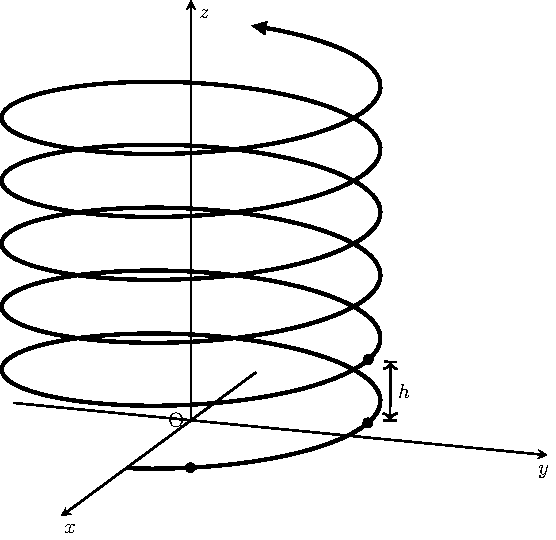
\includegraphics[width=\linewidth]{helix}
		\end{center}
	\end{minipage}
}
\QR{%
	Dessiner l'allure de la trajectoire.
}{%
	Cf.\ ci-dessus.
}
\QR{%
	Déterminer $h$ le pas de l'hélice, c'est-à-dire la distance selon
	l'axe (O$z$) dont sont séparés deux points successifs de la trajectoire
	correspondant à un même angle $\tt$ (modulo $2\pi$).
}{%
	Soit $t_0$ un instant quelconque. Un point à ce temps-là est tel que
	\[
		\left\{
		\begin{aligned}
			r(t_0)   & = R      \\
			\tt(t_0) & = \wt_0  \\
			z(t_0)   & = \a t_0
		\end{aligned}
		\right.
	\]
	Le premier point qui est au même angle $\tt$ mais avec $2\pi$ de plus se
	trouve donc à $t_1$ tel que
	\begin{align*}
		\tt(t_1)    & = \tt(t_0) + 2\pi
		\\\Lra
		\wt_1       & = \wt_0 + 2\pi
		\\\Lra
		\Aboxed{t_1 & = t_0 + \frac{2\pi}{\w}}
	\end{align*}
	On a alors
	\vspace*{-26pt}
	\begin{gather*}
		z(t_1) - z(t_0) = h = \a t_1 - \a t_0
		\\\Lra
		\boxed{h = 2\pi \frac{\a}{\w}}
	\end{gather*}
}
\QR{%
	Ce mouvement est-il uniforme~? À quelle condition est-il circulaire~?
}{%
	$\norm{\vf} = \sqrt{R^2\w^2+\a^2} = \cte$, donc il est uniforme. Il
	est circulaire ssi \fbox{$\a = 0$}.
}
\QR{%
	Déterminer les coordonnées cartésiennes de ce mouvement.
}{%
	En regardant dans le plan polaire, on trouve $x(t)$ et $y(t)$~:
	\begin{empheq}[box=\fbox, left=\empheqlbrace]{align*}
		x(t) & = R\cos(\wt)\\
		y(t) & = R\sin(\wt)\\
		z(t) & = \a t
	\end{empheq}
}

\end{document}
